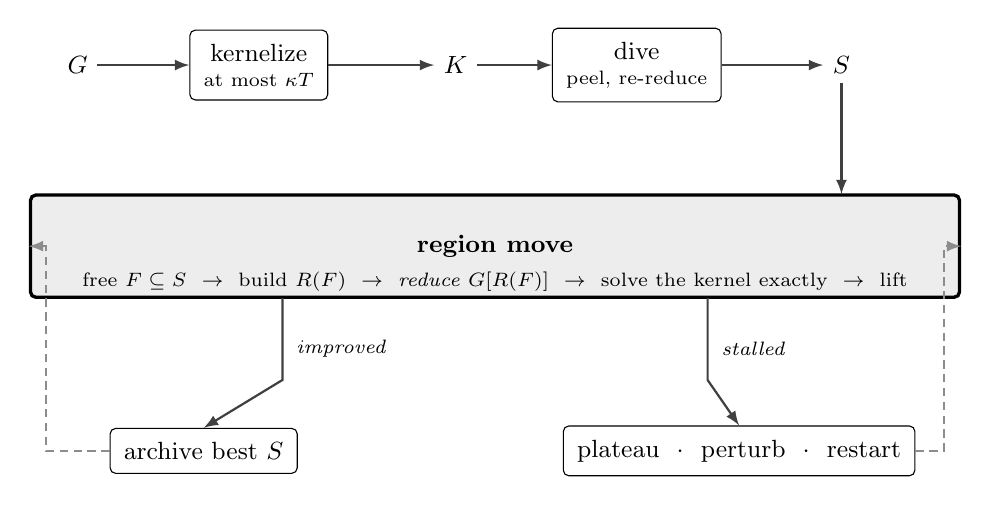
\begin{tikzpicture}[
  font=\small,
  box/.style={draw, rounded corners=2pt, align=center, inner sep=5pt, fill=white},
  core/.style={box, very thick, fill=black!7},
  flow/.style={draw, -latex, black!75, thick},
  back/.style={draw, -latex, black!45, thick, densely dashed},
  lbl/.style={font=\scriptsize\itshape, inner sep=2pt},
]

% ---------------- once, before the search ----------------
\node          (g)    at ( 0.0, 0) {$G$};
\node[box]     (kern) at ( 2.3, 0) {kernelize\\[-2pt]{\scriptsize at most $\kappa T$}};
\node          (k)    at ( 4.8, 0) {$K$};
\node[box]     (dive) at ( 7.1, 0) {dive\\[-2pt]{\scriptsize peel, re-reduce}};
\node          (s)    at ( 9.7, 0) {$S$};

\draw[flow] (g)    -- (kern);
\draw[flow] (kern) -- (k);
\draw[flow] (k)    -- (dive);
\draw[flow] (dive) -- (s);

% ---------------- the repeated part ----------------
\node[core, minimum width=118mm, minimum height=13mm] (move) at (5.3,-2.3)
  {\textbf{region move}};
\node[align=center] at (5.3,-2.75)
  {\scriptsize free $F\subseteq S$ \ $\rightarrow$ \ build $R(F)$ \ $\rightarrow$ \
   \emph{reduce $G[R(F)]$} \ $\rightarrow$ \ solve the kernel exactly \ $\rightarrow$ \ lift};

\node[box] (archive) at (1.6,-4.9) {archive best $S$};
\node[box] (escape)  at (8.4,-4.9) {plateau \ $\cdot$ \ perturb \ $\cdot$ \ restart};

% incumbent enters the loop
\draw[flow] (s) -- (9.7,-1.0) -- (9.7,-1.64);

% and the loop leaves it two ways
\draw[flow] (2.6,-2.96) -- (2.6,-4.0) -- (archive.north);
\node[lbl, anchor=west] at (2.7,-3.6) {improved};
\draw[flow] (8.0,-2.96) -- (8.0,-4.0) -- (escape.north);
\node[lbl, anchor=west] at (8.1,-3.6) {stalled};

% both paths return to the move
\draw[back] (archive.west) -- (-0.4,-4.9) -- (-0.4,-2.3) -- (move.west);
\draw[back] (escape.east)  -- (11.0,-4.9) -- (11.0,-2.3) -- (move.east);

\end{tikzpicture}
